\subsection{Simple Polygons}
\label{sec:warm-up}

Some of us may remember the following special case
of the Gauss-Bonnet theorem from middle school geometry.
Consider a simple polygon $P$, an example is shown in \figref{polygon}.

 \begin{figure}[htb]
         \centering
          \begin{subfigure}[b]{0.30\textwidth}
      		   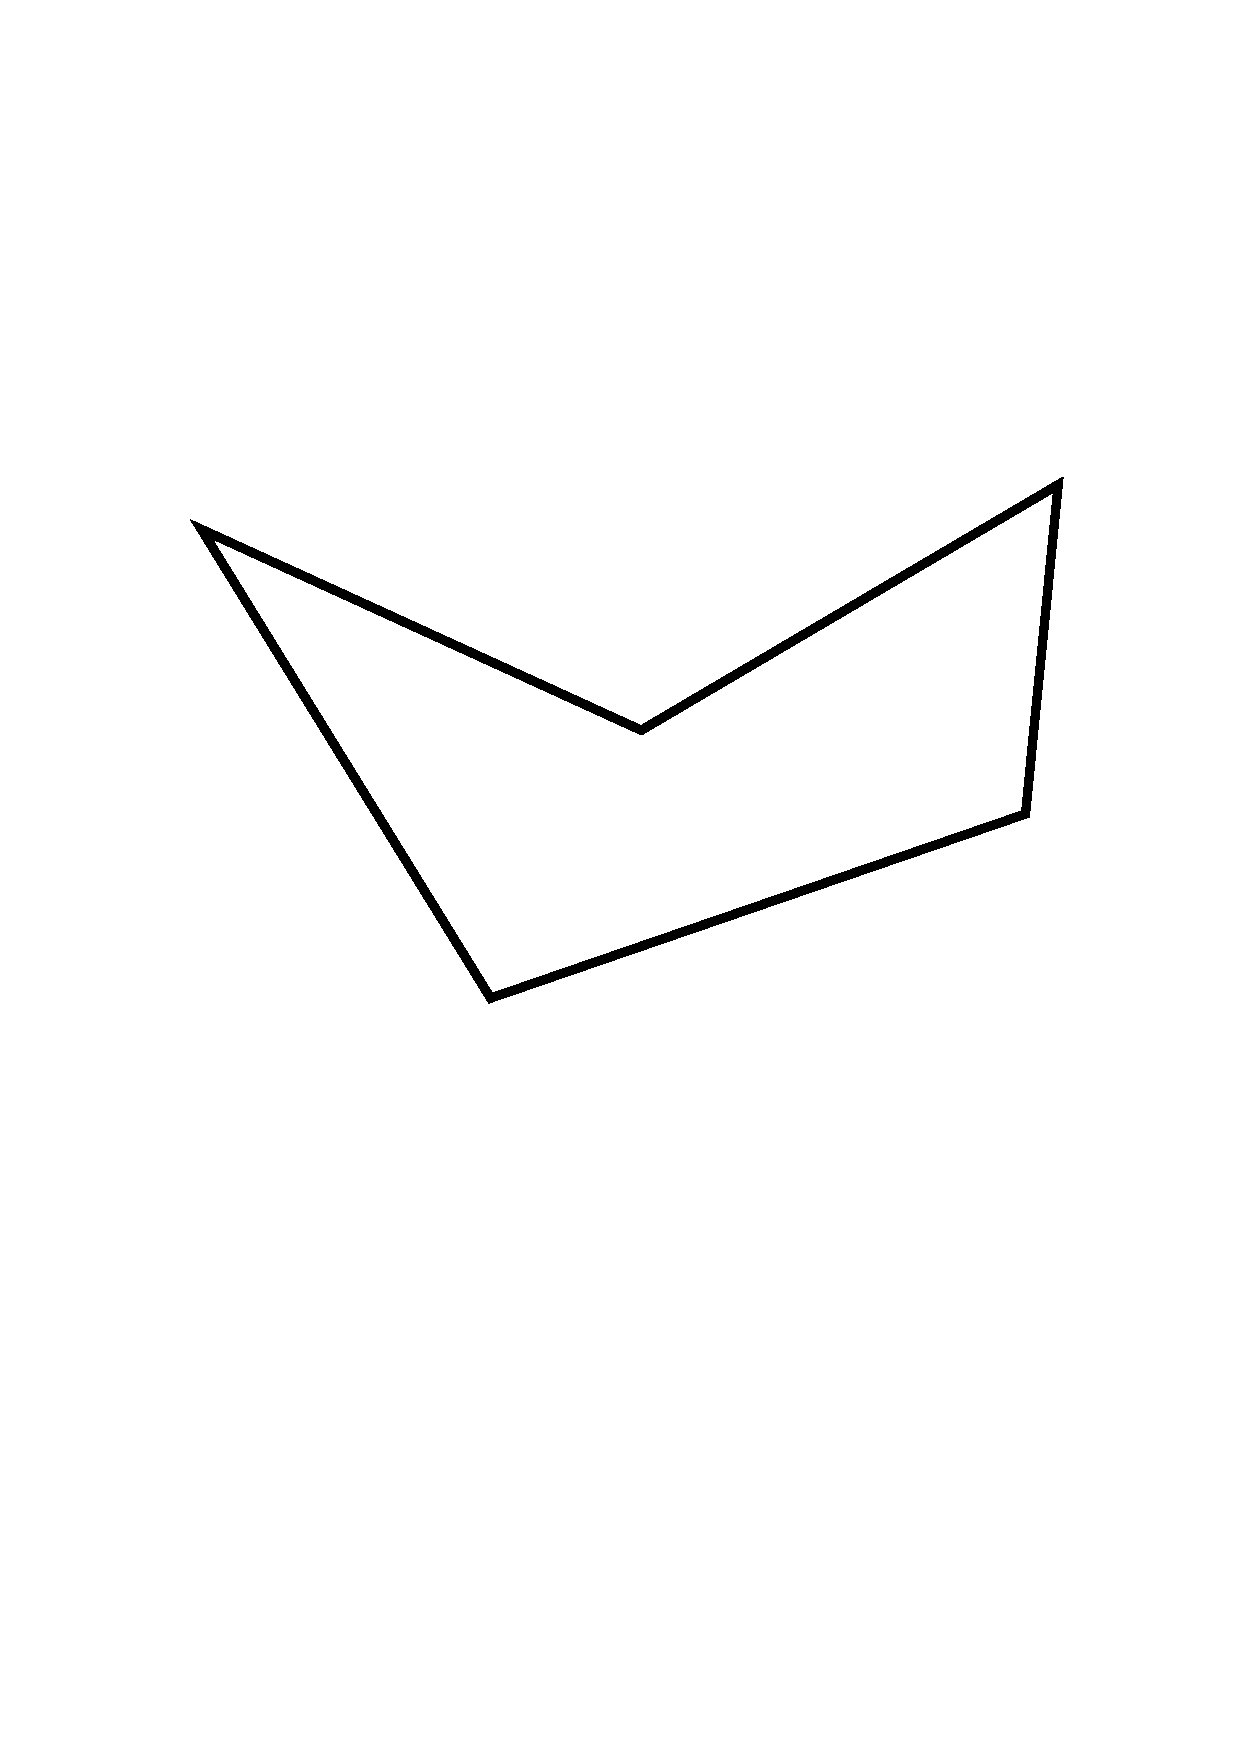
\includegraphics[width=\textwidth]{background/blank-polygon}
    		    \caption{A simple polygon.}
 		 \label{fig:polygon}
	 \end{subfigure}
	 \hspace{.5cm}
	 \begin{subfigure}[b]{0.25\textwidth}
       		  \includegraphics[width=\textwidth]{background/interior-exterior}
     		    \caption{Angles}
 		 \label{fig:interior-exterior}
       \end{subfigure}
        \hspace{.5cm}
     \begin{subfigure}[b]{0.27\textwidth}
       		  \includegraphics[width=\textwidth]{background/exterior-angles-polygon}
       		  \caption{Exterior angles.}
       		   \label{fig:exterior-angles}
         \end{subfigure}
		\caption{(\subref{fig:polygon}) A simple polygon $P.$
		(\subref{fig:interior-exterior}) The interior and exterior angles formed at a vertex.
 		 (\subref{fig:exterior-angles}) The sum of the exterior angles of a simple
		polygon is $2\pi$. Here
		$\beta_1+\beta_2+\beta_3+\beta_4+\beta_5=2\pi$ note that $\beta_4$ is negative.
 		\label{fig:simple-polygon}}
 \end{figure}

If we extend one of the sides of $P$ two complementary angles appear.
The angle inside $P$ is the \EMPH{interior} angle and the complement 
is the  \EMPH{exterior angle}. An example is shown in \figref{interior-exterior}.
We differentiate between turning left and right.
Vertices with interior angles  greater than $\pi$ are called \EMPH{reflex}, see \figref{exterior-angles}. 
At reflex vertices exterior angle is negative.



We now state a simple version of the Gauss-Bonnet theorem

\begin{theorem}[Gauss-Bonnet for Polygons in the Plane]\label{thm:simple-bonnet}
Let $P$ be a simple polygon in the plane with $n$  vertices,
interior angles $\{\alpha_1,\alpha_2,\ldots,\alpha_n\}$
and exterior angles $\{\beta_1,\beta_2,\ldots,\beta_n\}$ then
$$\sum_{i=1}^n\beta_i=2\pi$$
and 
$$\sum_{i=1}^n\alpha_i=\pi(n-2).$$
\end{theorem}


\begin{proof}

	We traverse a polygon and rotate $\beta_i$ at each vertex
	when we get back to where we started we will have preformed 
	one complete revolution so $\sum_{i=1}^n\beta_i=2\pi.$
	The exterior angles are complementary to the interior angles
	so for each $i$ we have $\beta_i=\pi-\alpha_i$  and using the first
	part of the theorem,  we have
	$\sum_{i=1}^n(\pi-\alpha_i)=n\pi -\sum_{i=1}^n\alpha_i=2\pi$. 
	Solving for $\sum_{i=1}^n\alpha_i$ gives the second part of the theorem.

\end{proof}


No matter how we position the vertices of our polygon,
if the boundary of the polygon stays closed and simple,
the sum the exterior angles will be $2\pi$.
Even this simple version of the Gauss-Bonnet theorem has powerful
consequences, as we now see in our first application, a proof of Pick's Theorem.







